

\chapter{Conclusion}

\label{chap:conclusion} 
\newcommand{\typetutor}{TypeTutor}

\graphicspath{{Figures/Conclusion}}

This thesis begins by establishing the context of our work within the field of programming languages, particularly emphasizing the significance of well-designed error messages. We explore the evolution of type-checking methods and techniques, followed by an in-depth discussion on utilizing Minimal Unsatisfiable Subsets (MUS) to report type errors and enhancing this with interactive features to handle multi-step type errors. Additionally, we examine the application of Minimal Correction Sets (MCS) to type error reporting, alongside strategies for debugging that involve multi-witness or multi-party type errors. Lastly, we discussed our design of a visual language for types, aimed at enhancing the programming experience and enriching the educational resources available for teaching and learning about types.

\section{Contributions}


\subsection{A categorization of type errors based on the structure of the evidence of a type error}


Drawing on insights from how human programmers perceive type errors and theories from constraint satisfiability research, we have developed a categorization framework for type errors. This framework helps identify three critical attributes of type errors, enhancing our understanding of strategic interventions to assist programmers in resolving these errors effectively.

\begin{itemize}
    \item {\textbf{Multi-step type errors} These errors involve a sequence of logical deductions, requiring programmers to probe multiple segments of the source code to forge a coherent reasoning chain. It is crucial to clearly present these clues and their interconnected relationships within the source code to support this reasoning process.}
    \item 
    \item{\textbf{Multi-witness type errors}  These errors present an inbalance in the evidence leading to two possible causes. Highlighting this discrepancy can guide programmers towards a more informed evaluation of the likely root causes, aiding in quicker resolution.}
    \item{\textbf{Multi-party type errors} These errors involve conflicts that present more than two potential possible types. They ften indicate the co-exsistence  of multiple underlying errors. Providing tools that can segment a multi-party type error into multiple type errors in simpler form allows programmers to tackle each error sequentially, simplifying the debugging journey.}
\end{itemize}


Following this classification, we delved into the three main systems we developed in our research—Chameleon (see Chapter \ref{chap:chameleon}), Goanna (see Chapter \ref{chap:goanna}), and GeckoGraph (see Chapter \ref{chap:gecko-graph}). Each system is designed to tackle some unique challenges associated with debugging type errors.

\subsection{Explaining Multi-step type erros and the chain of thought visualization}

\subsubsection{Technical Contribution - Chameleon}
We introduce Chameleon, an interactive Haskell type error debugging tool. Chameleon leverages Minimal Unsatisfiable Subsets (MUS) as its core type error representation. Its innovative approach transform MUS into a sequence of source code locations that are logically connected through unification operations. Externally, Chameleon enables programmers to explore these connections in step-by-step order. Additionally, Chameleon features an adaptive user interface, allowing programmers to tailor the information density of type errors according to their experience level.


\subsubsection{How programmers use type error slicing and chain of thought visualization to understand type errors}
We conducted three user studies to investigate the impacts of using debugging tools that support type error slicing and interactive exploration, such as Chameleon. Our findings reveal a notable improvement in debugging speed when employing type error slicing tools, particularly for complex tasks. Additionally, we observed a significant enhancement in debugging speed when programmers engaged with the interactive features of the tool, suggesting that active exploration of type errors can positively impact the debugging process.

\subsection{Iterate potential causes of multi-wintness and multi-party errors}

\subsubsection{Technical Contribution -- Goanna}

We contribute Goanna, a Haskell type error debugging tool that, like Chameleon, utilizes type error slicing to achieve comprehensive error localization.

Goanna sets itself apart by employing Minimal Correction Sets (MCS) to identify potential causes of type errors. It conducts an exhaustive analysis of all potential causes and corresponding actions required to resolve the type error. To avoid an overwhelming list of suggestions, Goanna employs a set of heuristics. These heuristics filter out less useful suggestions and prioritize potential causes based on their likelihood, ensuring a more focused and effective debugging experience.


\subsubsection{An evaluation of the effectiveness of MCS-based type debugging tools}
To assess the efficacy of MCS-based type error debugging strategies, we compiled a dataset of 86 Haskell programs sourced from various online discussions, embodying a wide range of type error scenarios. We evaluated Goanna's accuracy in identifying and resolving type errors in comparison to traditional compiler tools. Our findings affirm that Goanna consistently provide more accurate error cause identification compared to other tools. Goanna's heuristics not only effectively narrow down the list of possible causes but also consistently include the real cause in its top recommendations. Furthermore, although Goanna's processing speed is slower than that of conventional tools, it remains well within a range suitable for providing real-time feedback to programmers. 

\subsection{Visualizing Types}

\subsubsection{Technical Contribution -- GeckoGraph: A Visual Language for Polymorphic Types}

We introduce GeckoGraph, an innovative graphic notation system designed specifically for Haskell types. Unlike traditional type signatures, GeckoGraph utilizes a combination of colors, shapes, and symbols to highlight distinct type structures. GeckoGraph provides clear visual representation for type-level features such as type classes, parametric type variables, and high-rank types. When programmers need to compare two types — a frequent requirement in resolving type errors — GeckoGraph's visual grouping is often able to underscore subtle differences, providing clear graphical distinctions.

\subsubsection{An evaluation on how programmers use diagramtic type notation}

We conducted a large-scale user study to evaluate the effectiveness of GeckoGraph in enhancing the traditional text-based approach to type signatures. The study was designed as an interactive puzzle game incorporating gamification elements to stimulate participation and engagement. In total,  721 programmers of all expereience level participated the study. While the results showed that the use of GeckoGraph did not significantly impact the speed or overall success rate of solving problems, it proved signifiacant for supporting beginners to solve harder tasks more successfully. Additionally, feedback collected through a qualitative post-study survey was  positive, suggesting GeckoGraph is intuitve, non-intrusive, and helpful.

\section{Future Work}

In this section, we present three promising directions stemming from our existing work. Firstly, drawing upon our expertise gained from the development of Chameleon, Goanna, and GeckoGraph, we have introduced a novel debugging tool: \textit{TypeTutor}. We offer a glimpse into the envisioned interfaces and interactions within \textit{TypeTutor}, which have been shaped by insights from our existing tools and feedback from various user studies.

Secondly, we delve into the realm of rapid advancements in large language models (LLMs) and their evolving role in programming assistance, distinguishing them from conventional theory-based tools like Chameleon and Goanna. We explore the possibility of integrating traditional tools with LLMs to capitalize on their unique strengths and address their respective weaknesses effectively.

Lastly, we outline our plans to adapt our debugging tools for use in other programming languages, underscoring the potential advantages and challenges associated with this endeavor.

\subsection{\typetutor: Question-based Type Debugging}
Through observing programmers tackle type error challenges in a series of user studies, we have gained valuable insights into their approaches towards handling type errors and complex programming tasks. Armed with this understanding, we are inspired to introduce a novel debugging tool named \textit{TypeTutor}. \textit{TypeTutor} is designed to map debugging tasks into a series of questions that programmers naturally inquire about, while also helping programmers in deconstructing high-level debugging questions into actionable, granular queries.

This style of programming is often refered to as natual programmming environment \cite{Myers2004-fy}. Previous studies have underscored the benefits of employing a natural debugging interface, exemplified by tools like Alice~\cite{Conway2000-nn} and WhyLine~\cite{Ko2009-uf}. However, existing research predominantly concentrates on debugging runtime errors, neglecting exploration into type-level debugging.  Leveraging our experience with Chameleon, Goanna, and GeckoGraph, we envision meaningful progress in this domain.


\subsubsection{Why questions}

A fundamental aspect of debugging type errors involves asking questions such as "Why does the type error occur?" and "Why is the expected type \texttt{X}?" These "why" questions highlight gaps in a programmer's understanding, where a thorough explanation is in demand. \textit{TypeTutor} intelligently addresses this by displaying all relevant "why" questions when a programmer hovers over an expression of interest. Upon selecting a question, \textit{TypeTutor} promptly provides the corresponding detailed answer.



\begin{figure}[hbt]
  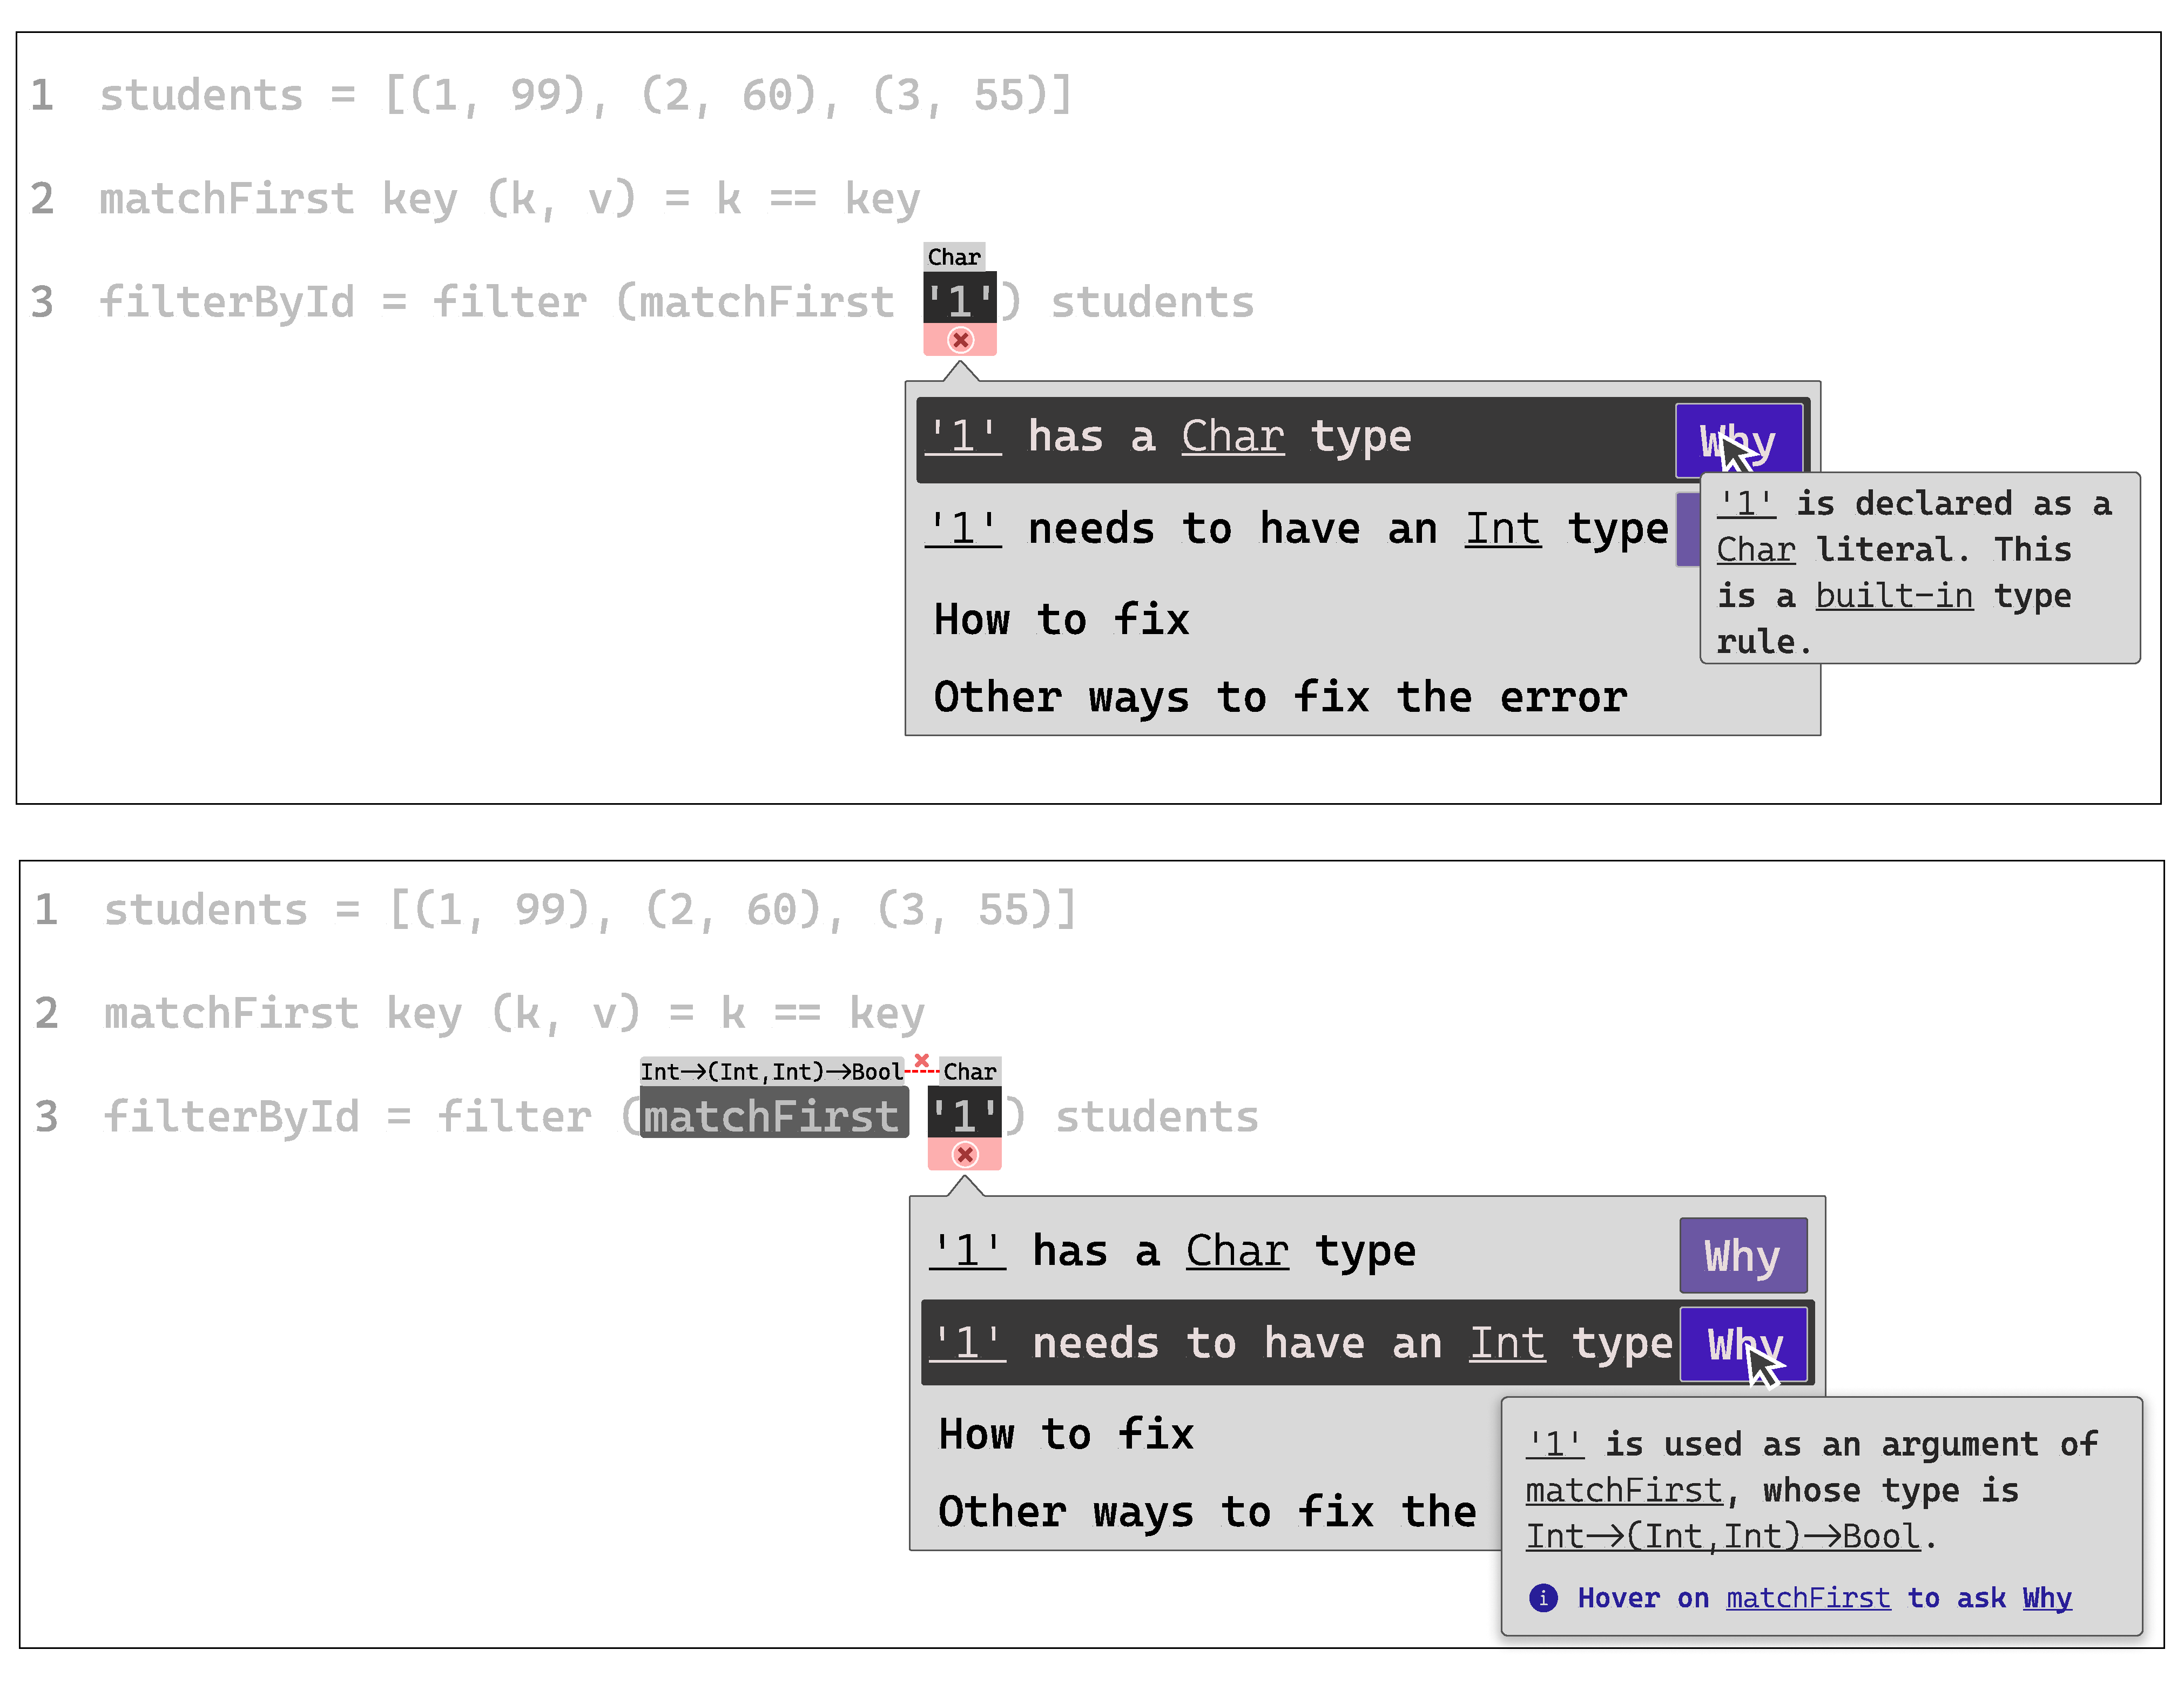
\includegraphics[width=\linewidth]{Why}
  \caption{
      Displaying a type error in level 1 explanation
    }
\end{figure}



\subsubsection{Follow-up questions: who watches the watchers}


In the context of debugging type errors, particularly multi-step type errors, it proves beneficial to enable programmers to incrementally uncover the underlying inference logic. \textit{TypeTutor} support this process by allowing programmers to ask follow-up questions. Typically, these questions build upon the responses to earlier inquiries. Follow-up questions in \textit{TypeTutor} facilitate tasks akin to the interactive debugging stpes in Chameleon. However, unlike Chameleon, \textit{TypeTutor} does not provide a separate interface for follow-ups. Instead, when a response includes the option for further inquiry, \textit{TypeTutor} provides a follow-up hint at the end of the answer, encouraging programmers to continue tracing the root cause. This integrated approach helps maintain a streamlined user experience while enabling deep exploration of type errors.


\begin{figure}[hbt]
  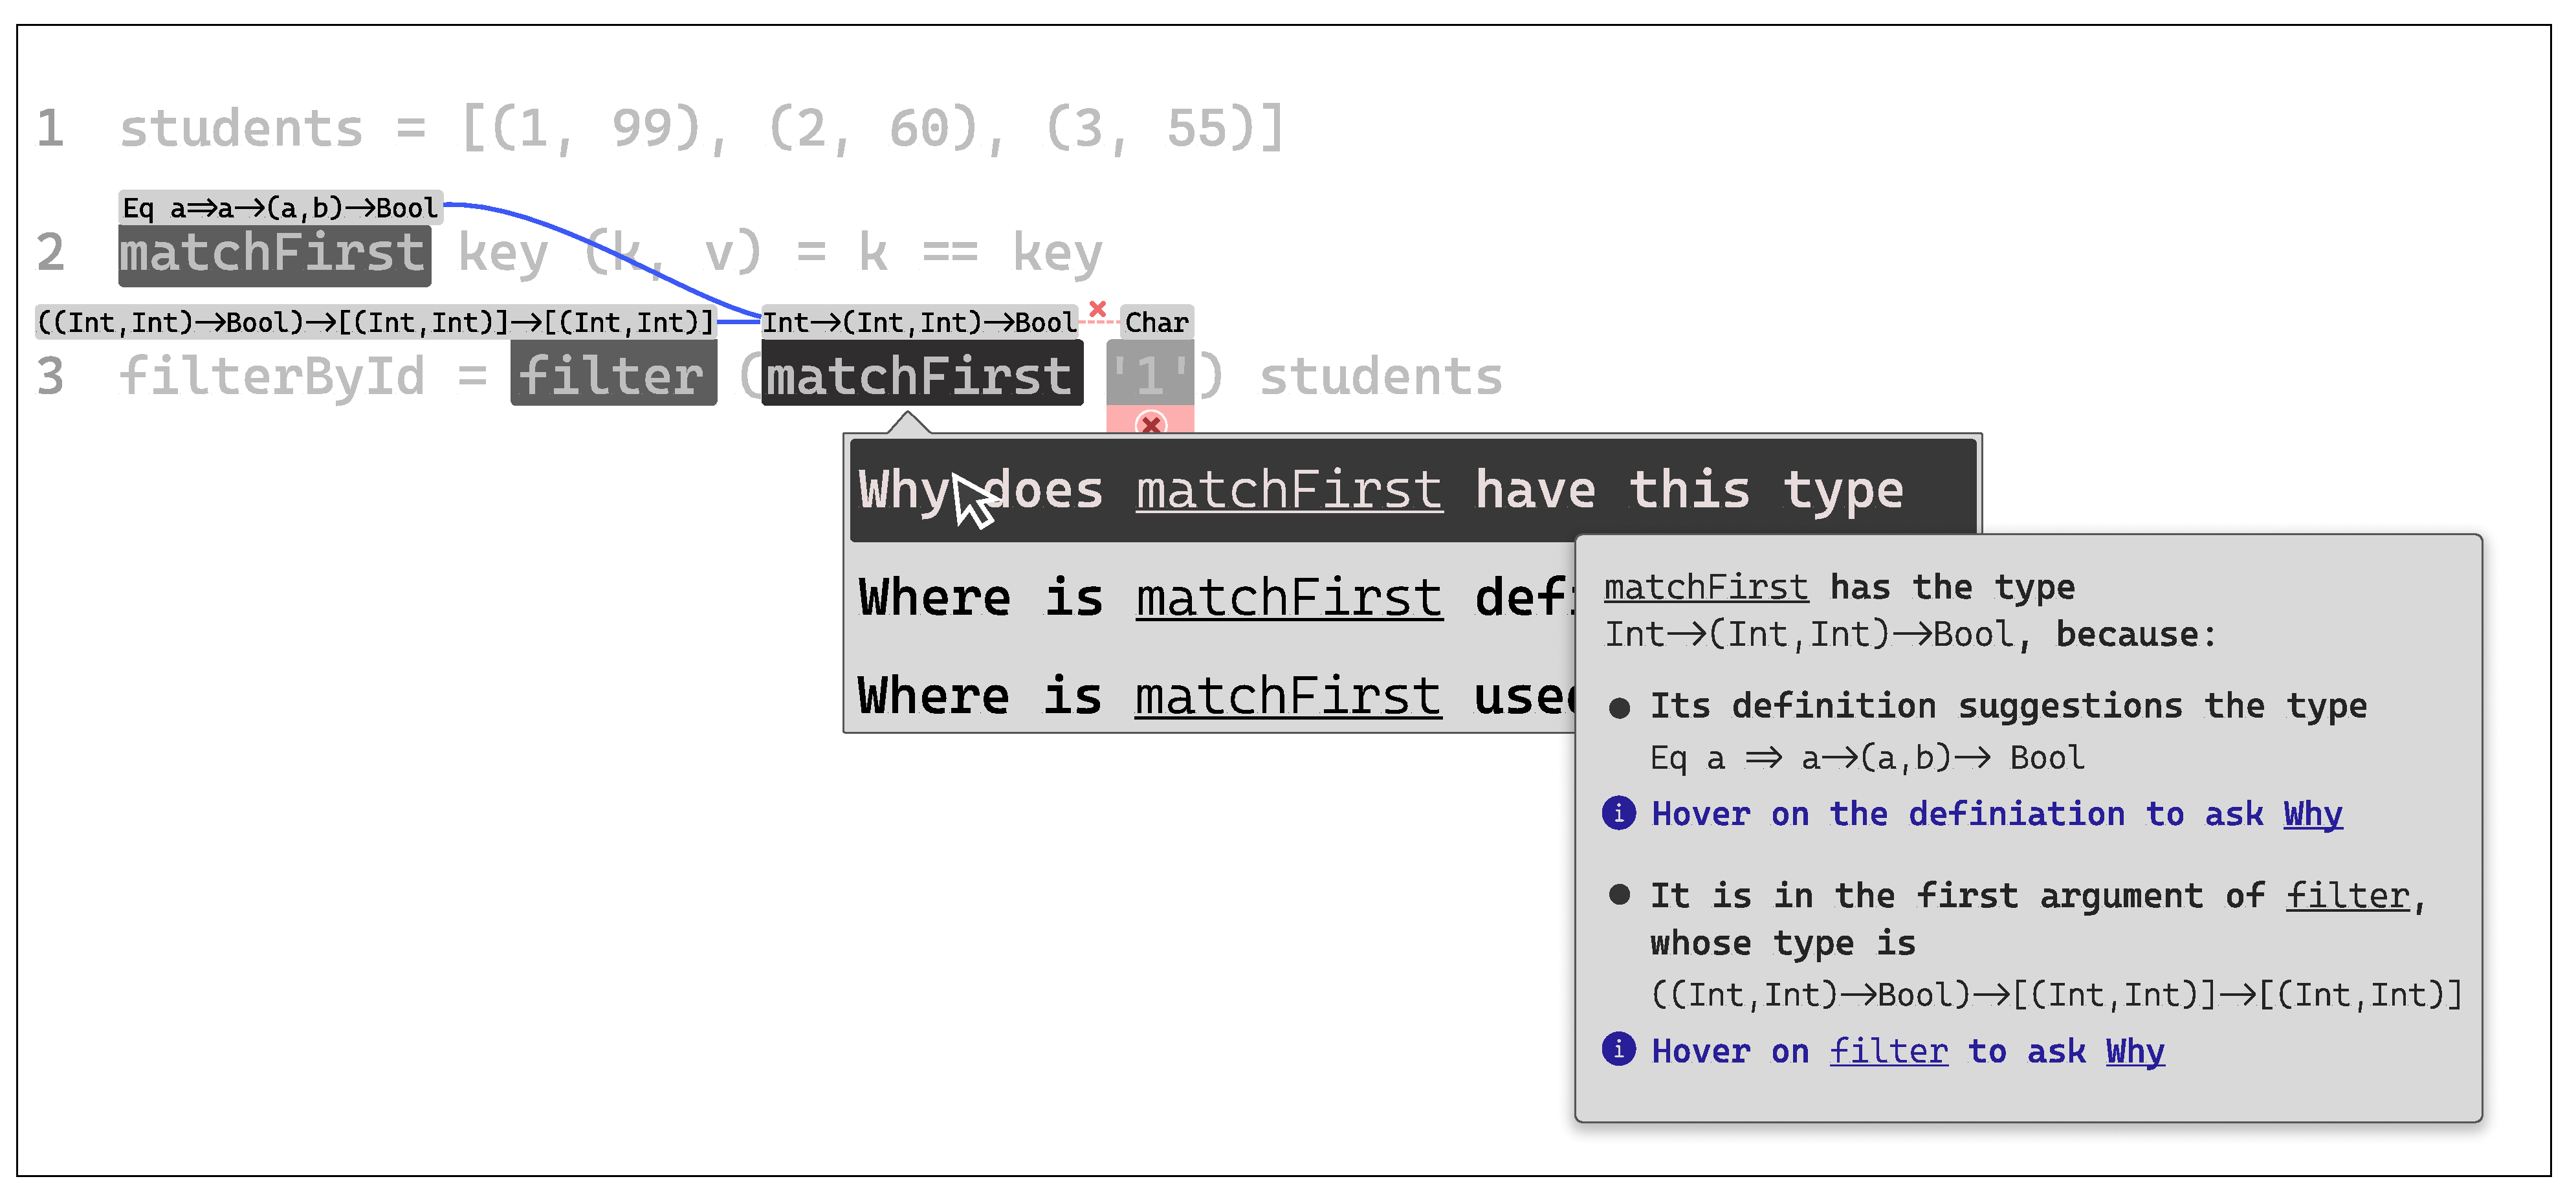
\includegraphics[width=\linewidth]{FollowUp}
  \caption{
      Displaying a type error in level 1 explanation
    }
\end{figure}
\subsubsection{How questions}

'How' questions in debugging focus on providing prescriptive guidance regarding program error. Such questions do not solely depend on logical precision; rather, they require the understanding of a programmer's knowledge gaps and the ability to deliver clear, followable instructions. \textit{TypeTutor} aids programmers by facilitating questions on how to rectify specific type errors. In Goanna, the analysis of Minimum Sufficient Syntax (MSS) can suggest the expected type for each possible correction. \textit{TypeTutor} advances this concept by offering examples of syntax changes tailored to these recommended types. 



\begin{figure}[hbt]
  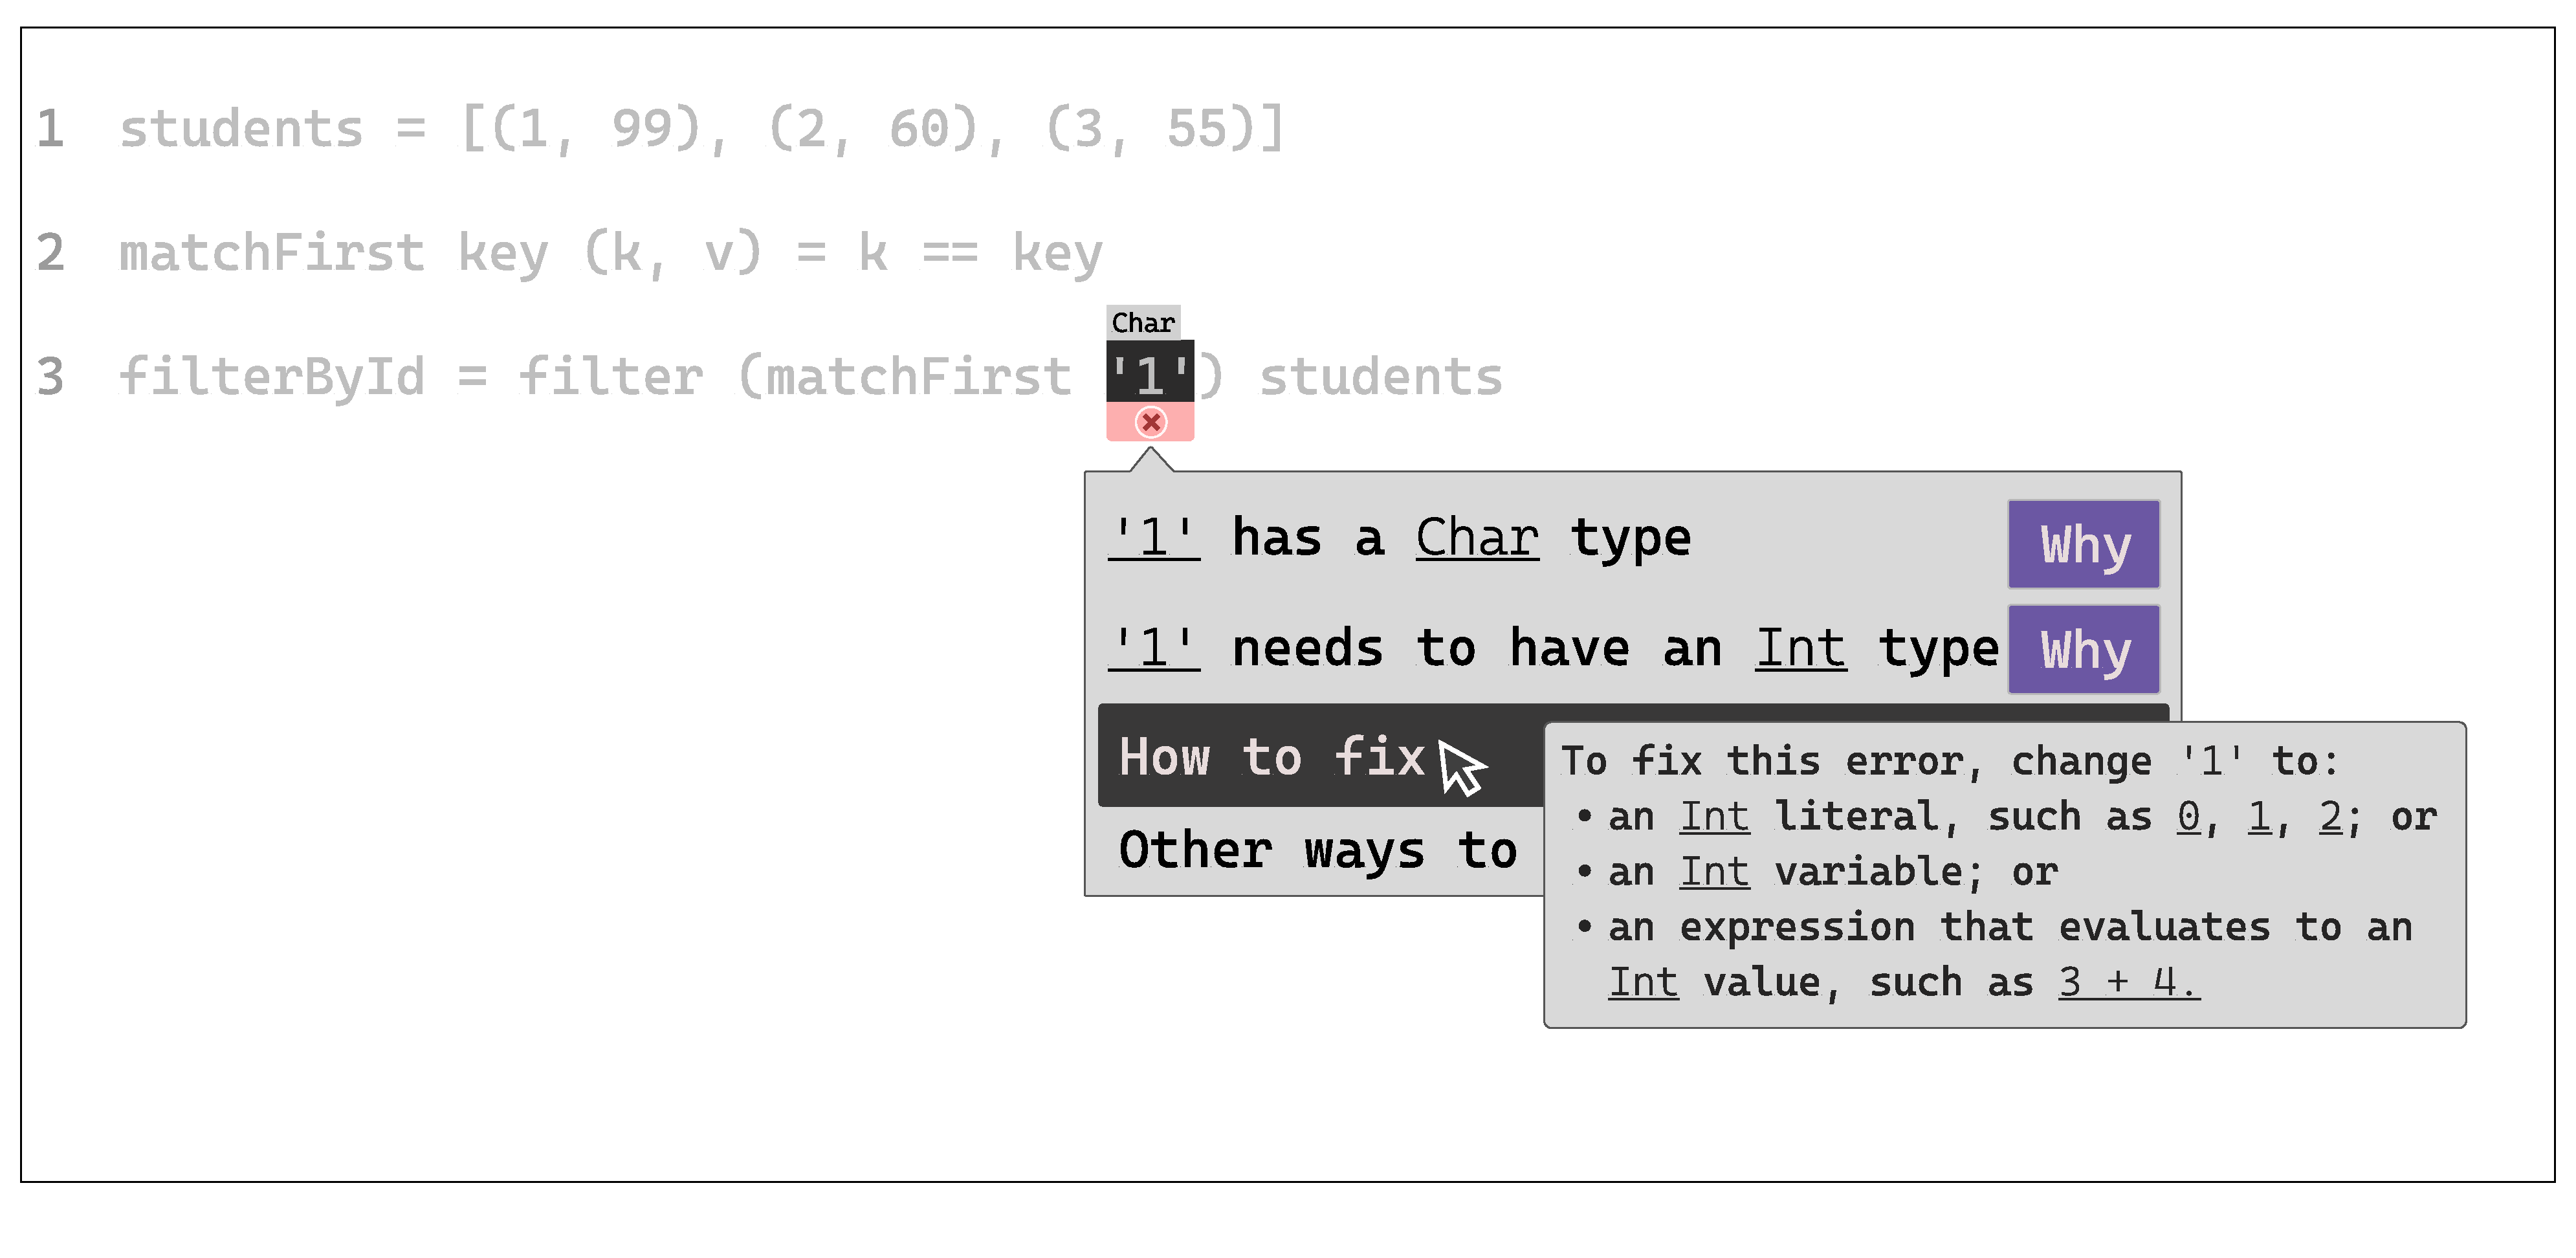
\includegraphics[width=\linewidth]{How}
  \caption{
      Displaying a type error in level 1 explanation
    }
\end{figure}

\subsubsection{What-if questions}
Finally, as we have identified, type errors frequently involve multiple potential causes and explanations. When integrated into a question-and-answer interface, the presence of multiple causes naturally prompts counterfactual questions such as "What are other ways that can cause this type error?" Recognizing this, \textit{TypeTutor} provides a natural and user-friendly interface for exploring various potential causes and solutions. This approach, while similar to the functionality offered by Goanna, features a more concise and intuitive interface for programmers to switch between different potential causes.

\begin{figure}[hbt]
  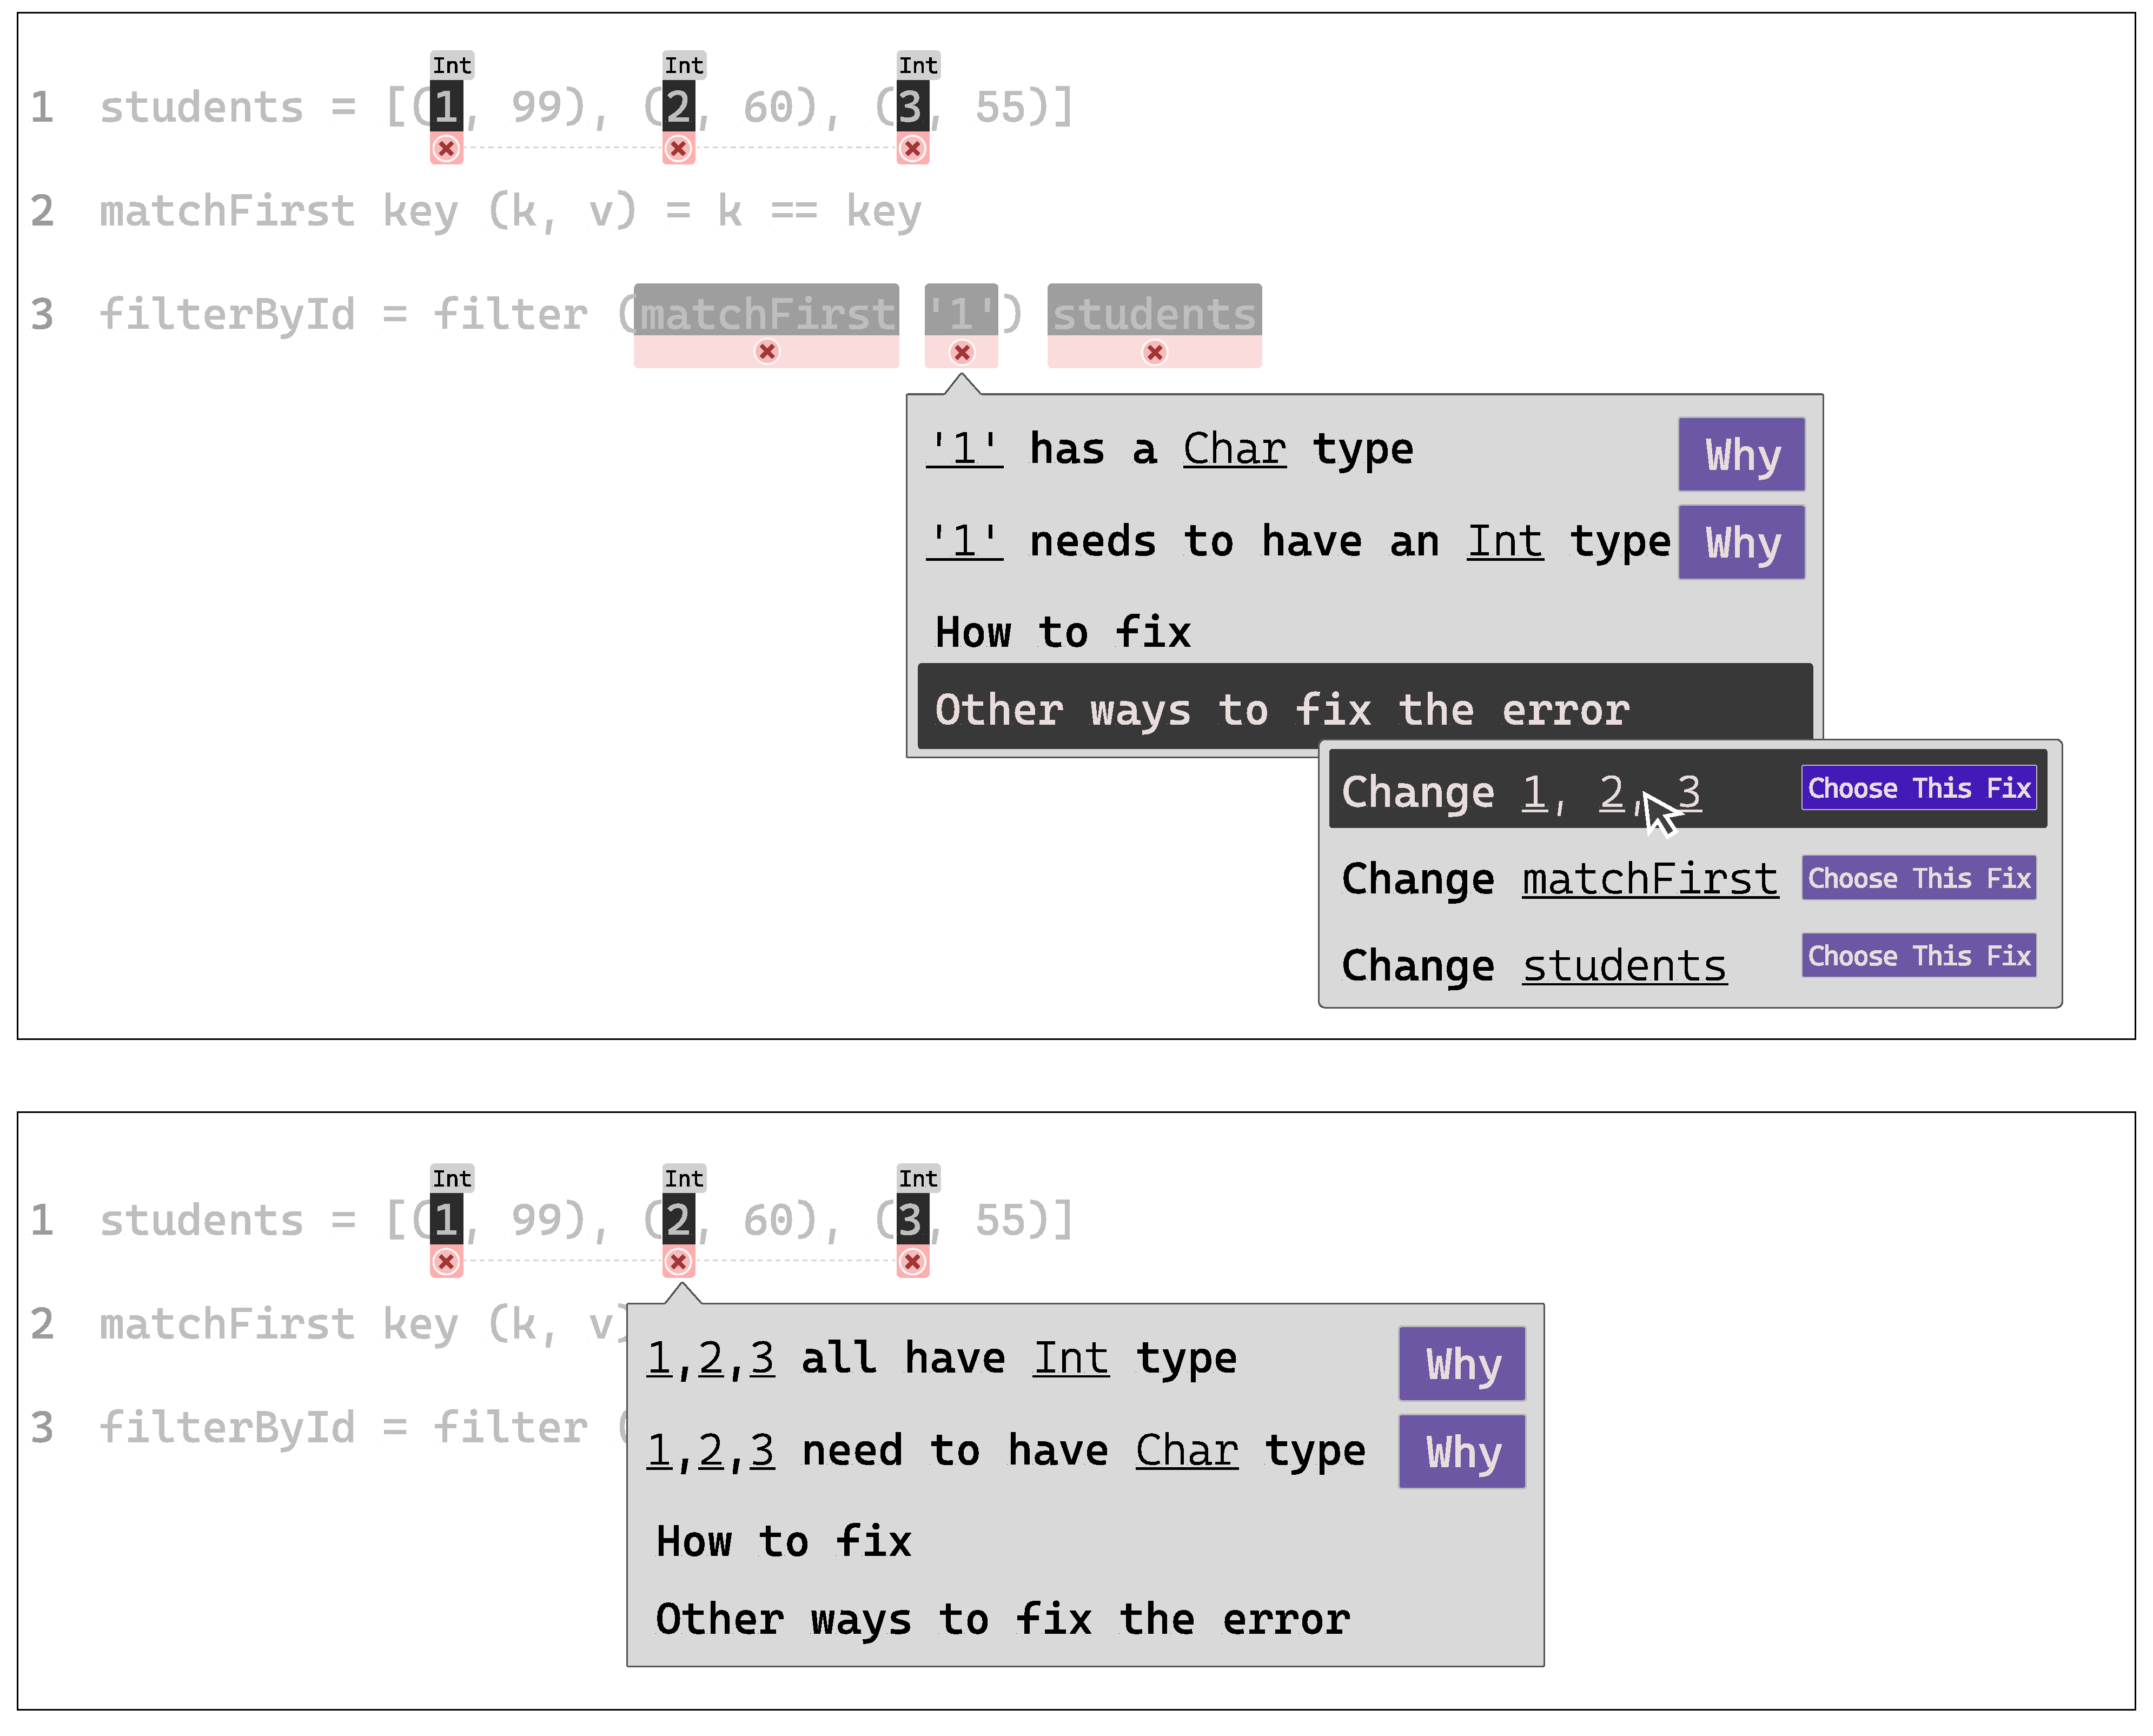
\includegraphics[width=\linewidth]{WhatIf}
  \caption{
      Displaying a type error in level 1 explanation
    }
\end{figure}


\subsection{Integration with Large Language Models}
At the time of writing this thesis, LLMs have been actively experiented to perform all kinds of tasks that require human creativity. This of course include programming. Many attempts to use LLMs to replace programming and free programmers for higher level thinkings. This development in tangential with our objective of explaining type errors and reasoning about the logic of type inference. 

\begin{figure}[hbt]
  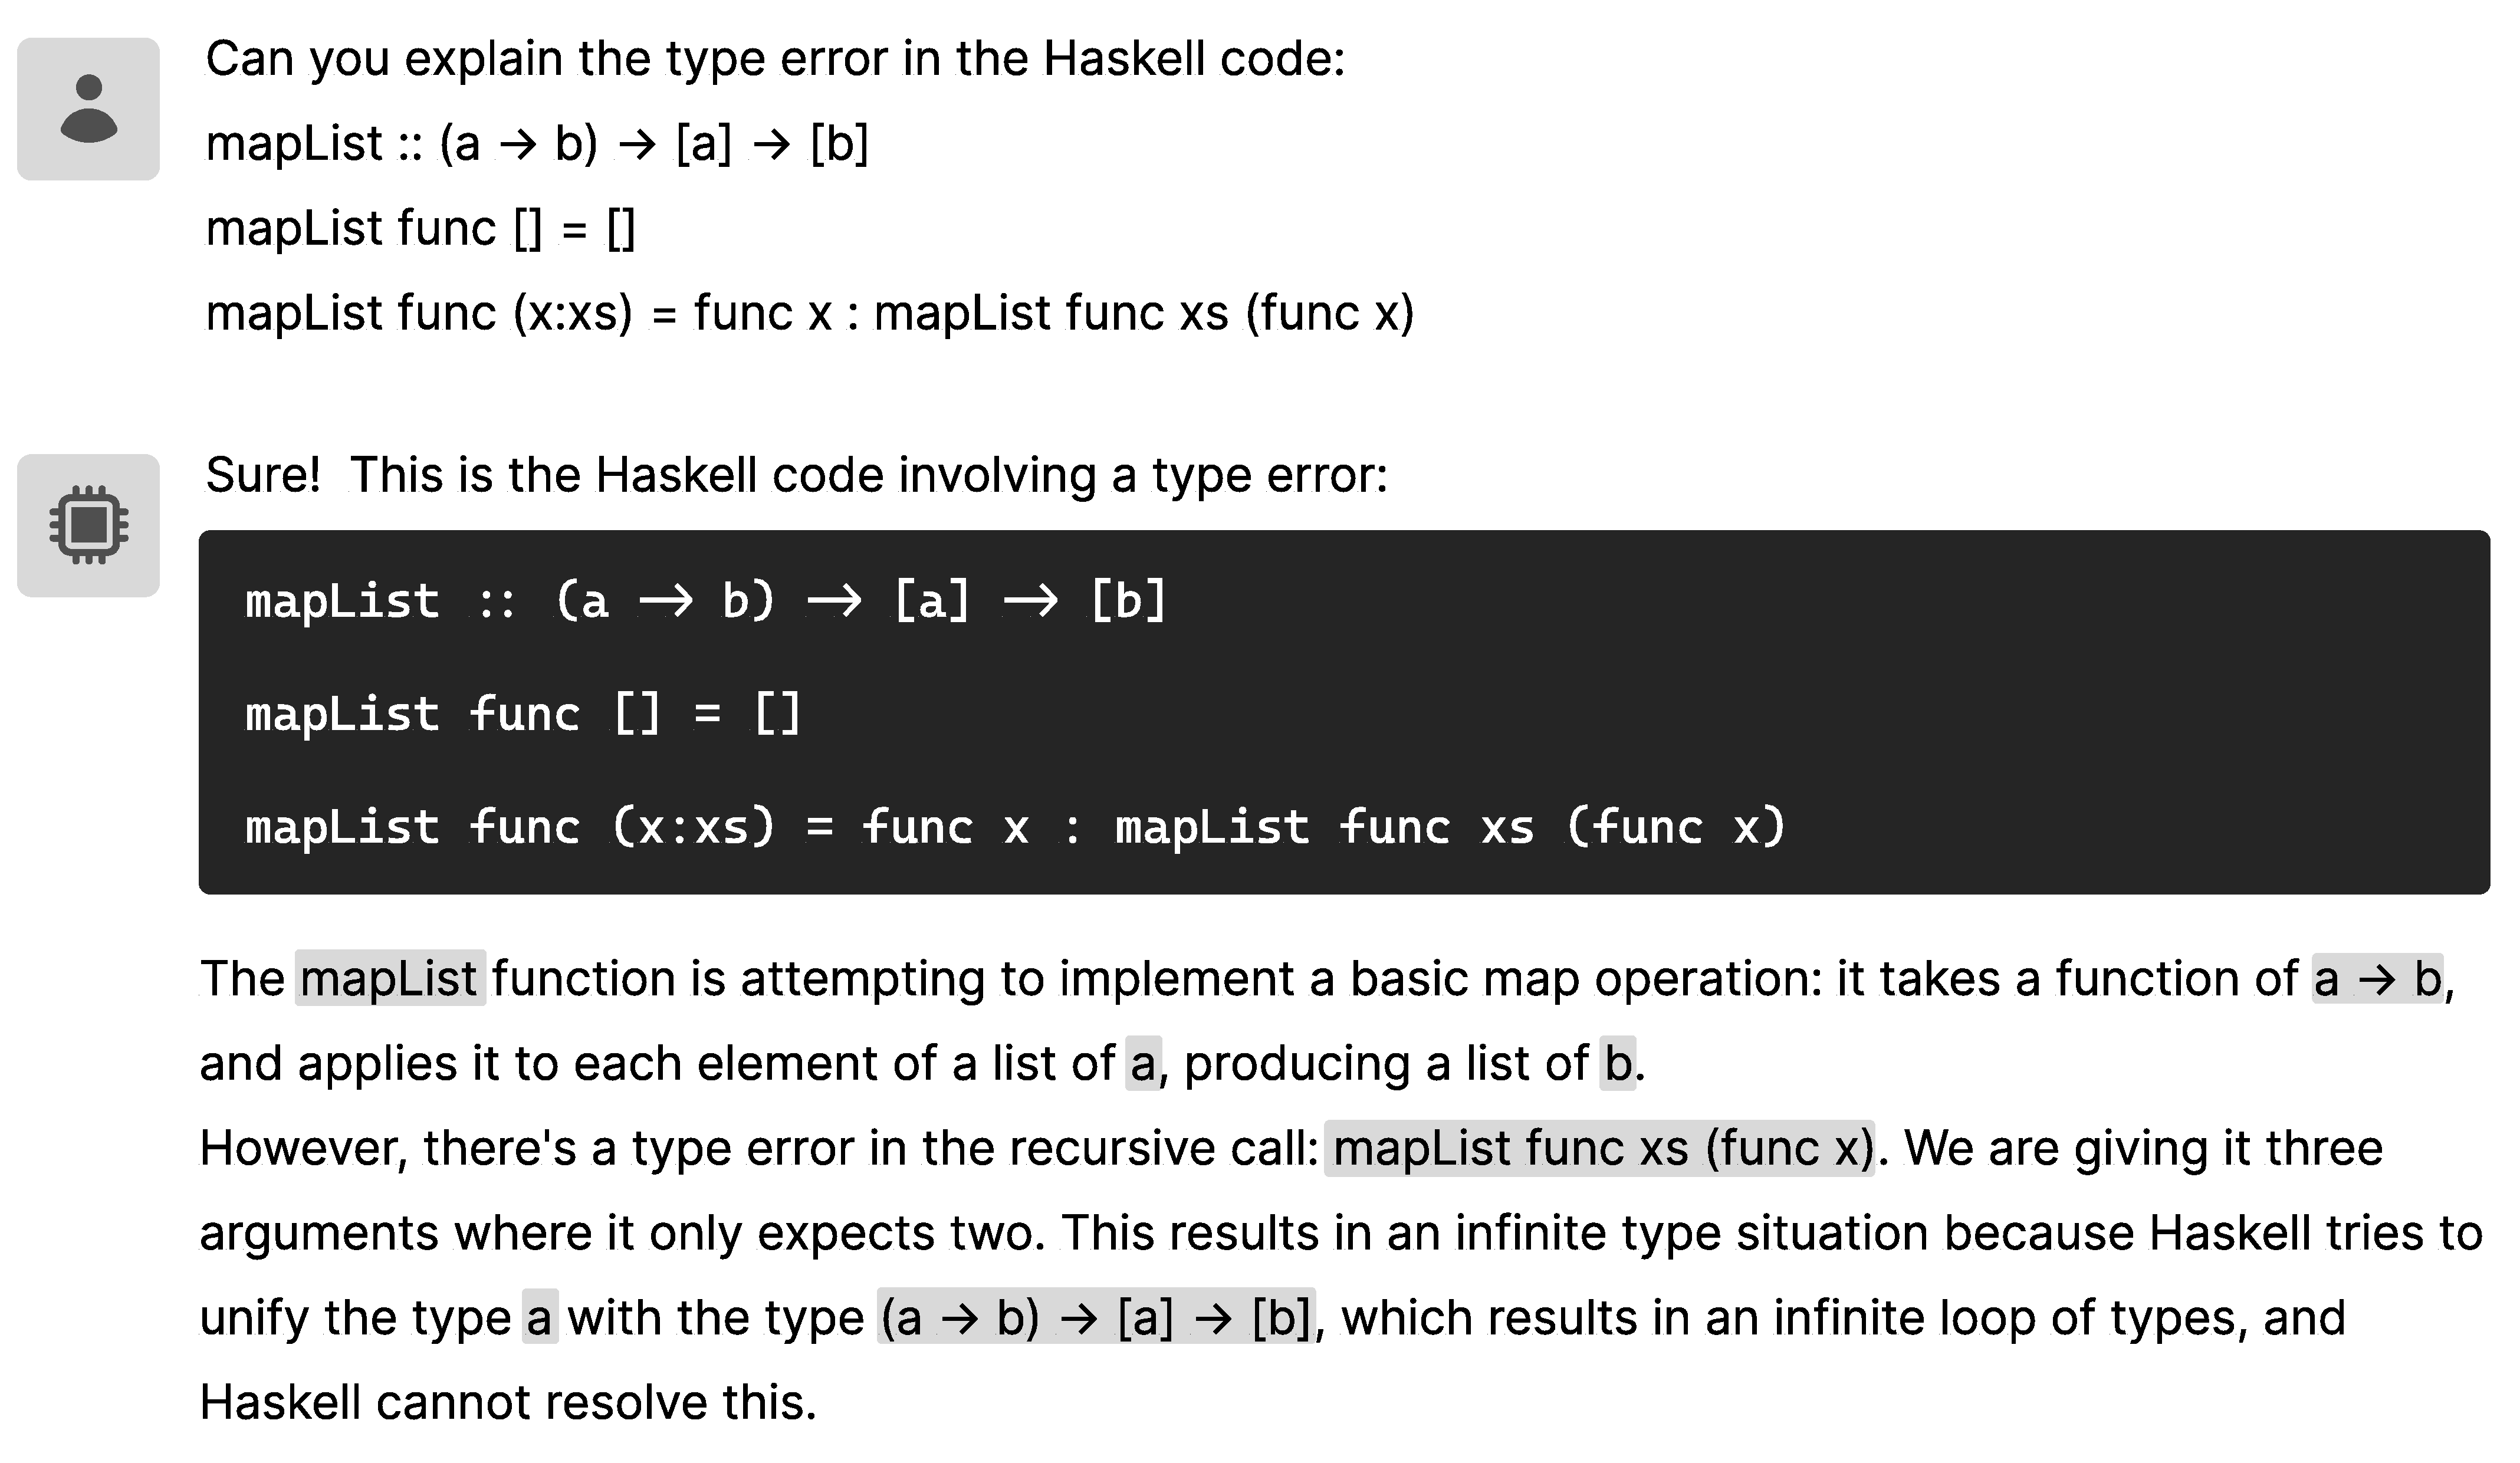
\includegraphics[width=\linewidth]{LLM}
  \caption{\label{fig:llm}
    }
\end{figure}

While LLMs have shown capability in recognizing basic errors, they often display a limited understanding of type theories and multi-step reasoning ability. On the error in Figure 3,although provided a correct fix, ChatGPT 3.5 claimed “The type error occurs because the matchFirst function expects a tuple (k, v) as its second argument, but when using it with filter, the second argument of filter should be a list. You're trying to apply filter to a function (matchFirst '1') and a list (students), but matchFirst '1' expects a tuple, not a list”, illustrating a fundamental lack of understanding of higher order types, and certainly not a correct explanation.

\begin{figure}[hbt]
  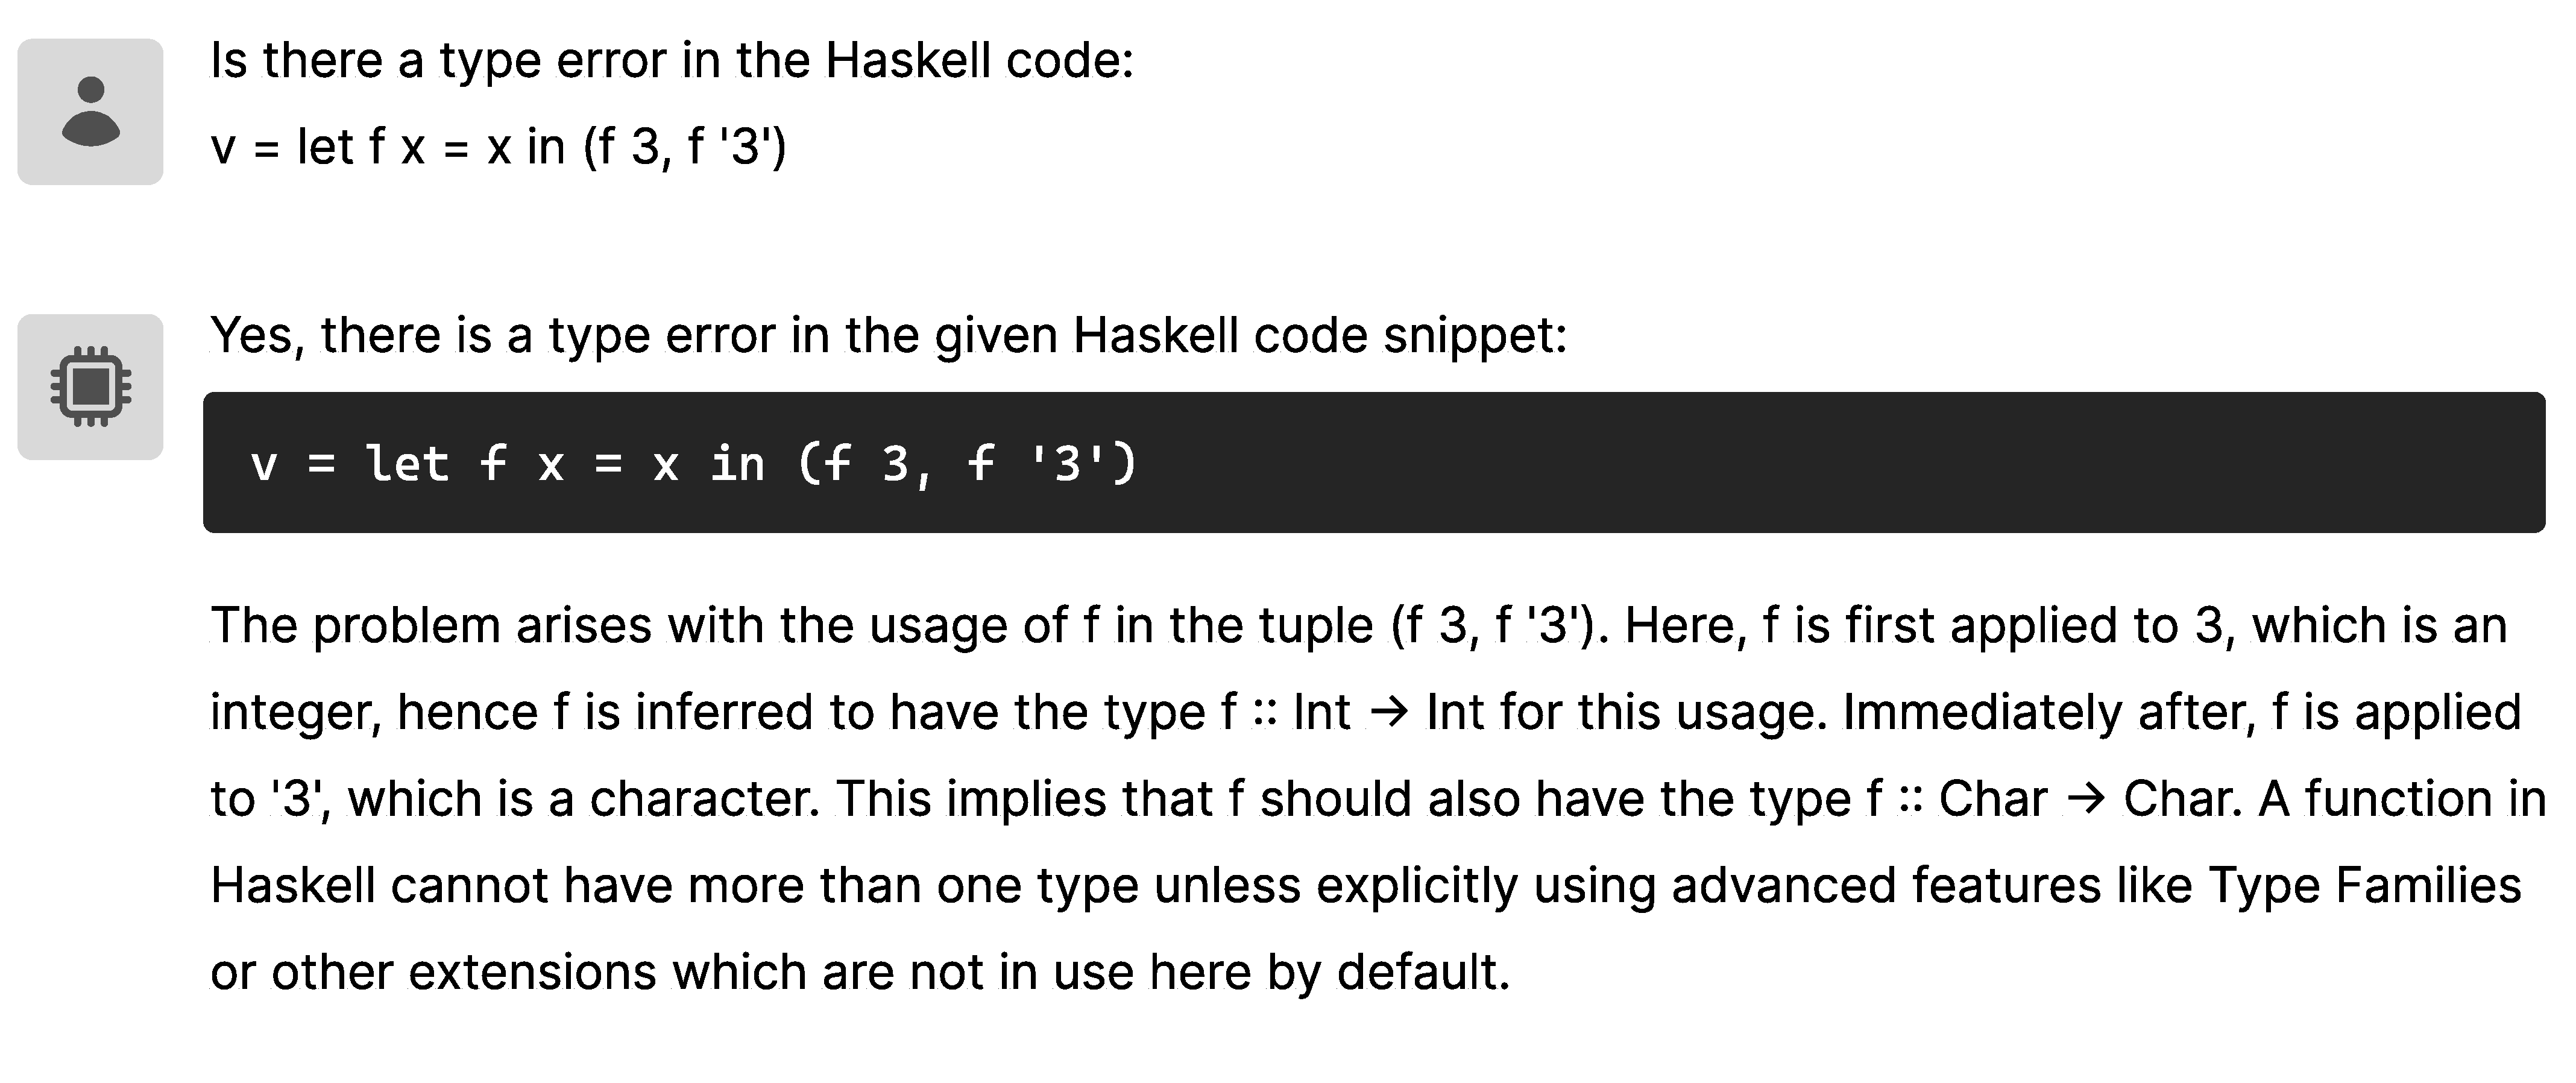
\includegraphics[width=\linewidth]{LLM2}
  \caption{\label{fig:llm2}
    }
\end{figure}

When tested with the prompt "is there a type error in the Haskell code: v = let f x = x in (f 3, f '3')", most LLMs incorrectly reported yes. LLMs can give wrong explanations, find type errors that don't exist, unlike tools like GHC, Helium and Goanna. While there is clearly a role for their usage in programming assistance, they do not “reason” about types and hence are not trustworthy.

While LLMs are getting more and more accurate everyday, some doubt whether they will ever become as reliable as theory-based tools. We believe in the great potential of integrating LLMs with existing theory-based tools, such as Chameleon and Goanna. This integration could enhance the LLMs' performance by aligning their operation with accurate theoretical guides, or by utilizing their strengths in areas where traditional tools fall short, like suggesting syntactical improvements. This synergy could lead to more robust programming assistance using both types of tools.

\itemize{
  \item{Code Generation and Validation: LLMs could generate code which Goanna then checks for errors. Detected errors could be fed back to the LLMs for corrections, enhancing both the efficiency and accuracy of code development.}
  \item {Error Tutoring and Resolution: Goanna could identify errors in manually written code, with LLMs suggesting syntax corrections. This combines Goanna's precise error detection with the LLMs' ability to generate effective syntax changes, surpassing traditional tools in this domain.}
}

\subsection{Support for Other Languages}
\subsubsection{Motivation}
While Haskell is the ideal platform for studying programming languages and type systems, we strongly believe a vital course of development of our research is to extend our tools to other languages. In recent years, we have observed the type system issues have infiltrated into many mainstream language like Rust and TypeScript. If we can successfully support these language with debugging features provided in our tools, it will help us reach a much broader audience. It will also help testing our tools in more different projects in terms of style and scale.   This would also help us gather broader feedback.   

Many of  our work are already designed with other languages in mind. For instance, GeckoGraph, as a design is not limited one language, different languages can provide their own implemntations. It is a bit complicated with Chameleon and Goanna. The analysis of unsatisfiable constraints is universal across all languages, so is the theories and implemntations for enumeraing MUSes and MCSes.
That is to say, the underlying theories of Chameleon and Goanna are already supporting different languages. However, two challenges arrise from adopting these tools. First is the constraint generation. It is necessary to create constraint generation rules for each language, and this may require non-trivial changes based on the type-level features are present in the language. One example is that Haskell's functions are all curried, a feature not found in languages like TypeScript. In TypeScript, functions are defined with a fixed arity, with the option to overload. This differnce means that we can detect a type error if a function is applied to fewer arguments that it is defined, which is not the case in Haskell.   Second, the display of type error may need subtle adjustments for different languags. Special visualization techniques may need to be invented for ideas not found in Haskell, such as subtyping (TypeScript) and lifetime(Rust). 



\section{Final words}

Programming languages is a fascinating topic. It certainly is my favorourte in computer science for it combines ideas from vastly diffent schools. Among them, functional programming and static typing has been some of the brilliant ideas in programming languages. My research is centered on exploring why are type errors hard and how to make them paletable. The approaches we use are largely based on constrint satisfiability theoris. This including analysing MUS (Chameleon) and MCS (Goanna). We also use a lot of human-centerd research methods, formative studies, user studies, rapid prototyping, among others. We firmly believe it is a useful direction for programming language research. We hope the our study will be useful reference for brilliant future studies to come.




